\section{Spread impact in price response functions}\label{sec:spread_impact}

When we calculate the price response functions, the signal of the response
depends directly on the analyzed stock. Thus, even if the responses functions
are in the same scale, their values differ from one to another. We choose the
spread \cite{reg_and_irreg} to group 524 stocks in the NASDAQ stock market for
the year 2008 in physical time scale, and check how the average strength of the
price self-response functions in physical time scale behaved for this groups.
For each stock we compute the spread in every second along the market time.
Then we average the spread during the 253 business days in 2008. With this
value we group the stocks.

We used three intervals to select the stocks groups ($s<0.05\$$,
$0.05\$ \le s <0.10\$$ and $0.10\$ \le s <0.40\$$). The detailed information of
stocks, the spread and the groups can be seen in Appendix
\ref{app:spread_impact}. With the groups of the stocks defined, we averaged the
price response functions of each group.

In Fig. \ref{fig:spread_impact} we show the average response functions for
the three groups. The average price response function for the stocks with
smaller spreads (more liquid) have in average the weakest signal in the figure.
On the other hand, the average price response function for the stocks with
larger spreads (less liquid) have in average the strongest signal. According to
the results described in Sect. \ref{sec:response_functions_def} and
\ref{sec:response_functions_imp}, the average price response functions for all
the groups follow the increment to a maximum followed by a decrease in the
signal intensity.

\begin{figure}[htbp]
    \centering
    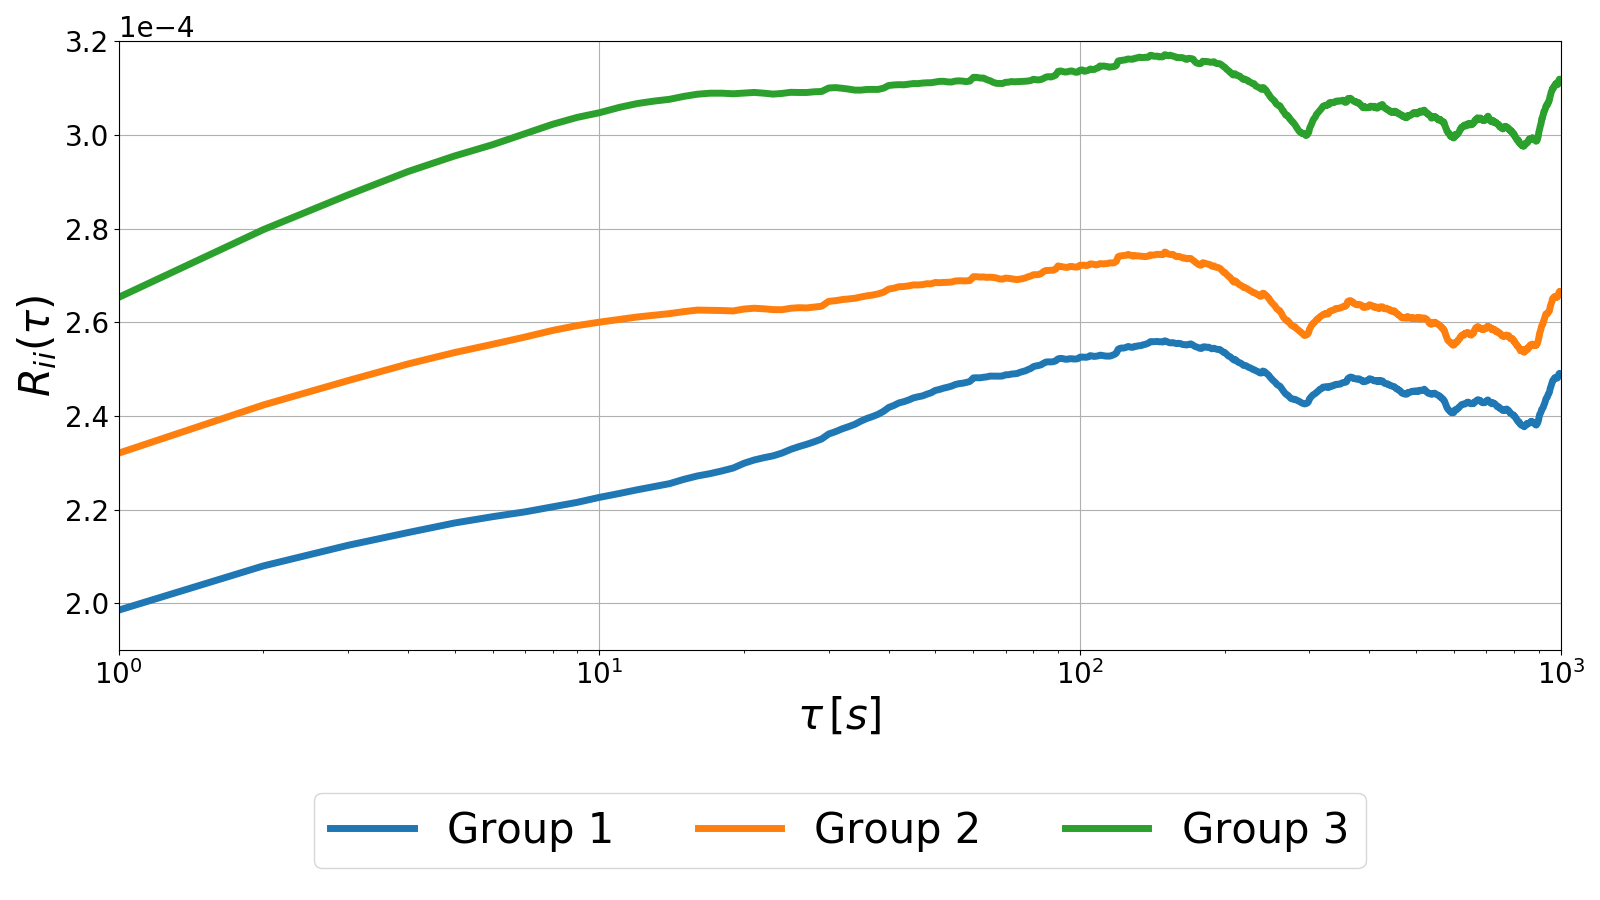
\includegraphics[width=\columnwidth]{figures/06_spread_impact_2008.png}
    \caption{Average price self-response functions
             $R^{\left(p\right)}_{ii}\left(\tau\right)$ excluding
             $\varepsilon^{\left(p\right)}_{i}\left(t\right) = 0$ in 2008
             versus time lag $\tau$ on a logarithmic scale in physical time
             scale for 524 stocks divided in three representative groups.}
    \label{fig:spread_impact}
\end{figure}

The strength of the price self-response function signals grouped by the spread
can be explained knowing that the response functions directly depend on the
trade signs. As long as the stock is liquid, the number of trade signs grow.
Thus, at the moment of the averaging, the large amount of trades, reduces the
response function signal. Therefore, the response function decrease as long as
the liquidity grows. And as stated in the introduction the spread is negatively
related to trading volume, hence, firms with more liquidity tend to have lower
spreads.

Finally, an interesting behavior can be seen in Fig. \ref{fig:spread_impact}.
Despite each stock has a particular price response according to the returns and
trade signs, the average price response function for the different groups
seems to be quite similar. As all the analyzed stocks come from the same market
we can infer that the general behavior of the market affect all the stocks,
influencing in average a group response.